\documentclass[12pt]{article}

\usepackage{sbc-template}

\usepackage{graphicx,url}

\usepackage{amssymb}
\usepackage{amsmath}

\usepackage{float}
\usepackage[utf8]{inputenc}  
     
\sloppy

\title{GERAÇÃO DE DADOS SINTÉTICOS UTILIZANDO MODELO DE TRIAGEM AMIB/ABRAMEDE}

\author{Alison Sassi\inst{1} \and Gustavo Spiess\inst{2} }

\address{Departamento de Ciências Exatas e Engenharias\\
Universidade Regional do Noroeste do Estado do Rio Grande do Sul
  (UNIJUÍ)\\
  Rua do Comércio, 3000, Universitário -- 98700-000 -- Ijuí -- RS -- Brazil
  \email{alisonsassij@gmail.com \and gustavospiess@gmail.com}
}

\begin{document}

\maketitle

\section{RESUMO}

Nos últimos cem anos, a maior pandemia ocasionada pela doença da COVID19 em 2020 foi a mais mortal, presenciamos um cenário de colapso da estrutura hospitalar pública, falta de leitos, de respiradores e profissionais da saúde. Os leitos de Unidade de Terapia Intensiva (UTI) foram alocados na sua totalidade, portanto, médicos tiveram um desafio de entender a prioridade de um paciente em um leito de UTI devido a alta demanda, ocasionando em problemas psicológicos, muitas vezes sendo uma escolha baseada no emocional do médico. Durante esse período, médicos realizaram uma decisão de quem ocupava um leito disponível, utilizando protocolos de triagem e guias criados por vários lugares do mundo, para minimizar a quantidade de mortes, dentre eles o protocolo publicado em 2020 pela Associação de Medicina Intensiva Brasileira (AMIB). Este artigo tem por objetivo descrever o modelo publicado pela AMIB utilizado para a triagem, explicar a forma que as variáveis foram extraídas e demonstrar a forma da geração de dados sintéticos, com a intenção de validação dos critérios sugeridos.

\textbf{Palavras-chave:} Unidade de Terapia Intensiva (UTI); Escassez de leitos hospitalares; Auxílio para médico na triagem;. Protocolo AMIB/ABRAMEDEE. Escala SOFA.

\section{ABSTRACT} 
\textbf{Keywords:} Intensive Care Unit (ICU). Shortage of hospital beds. Medical assistance. Hospital management. Protocol.

\section{INTRODUÇÃO}

Em 31 de dezembro de 2019 foi reportado casos de uma grave pneumonia de origem desconhecida na província de Hubei em Wuhan/China para a Organização Mundial de Saúde (OMS), a qual foi nominada de "Covid-19" para uma síndrome respiratória aguda grave causada pelo novo vírus identificado Sars-CoV-2, sendo uma doença facilmente contagiosa, transmitida por gotículas, recebendo mutações constantemente \cite{sa2020especial}. 

Em fevereiro do ano de 2020 foi registrado o primeiro caso no Brasil, com o passar dos dias os casos aumentaram exponencialmente no mundo todo, alcançando um nível de ameaça global muito elevado, em poucos dias todos os estados do Brasil tinham centenas de pacientes com a doença, ocasionando em internações em leitos de UTI, se tornando a maior pandemia dos últimos cem anos.

No Brasil os leitos de Unidade de Terapia Intensiva (UTI)  são historicamente escassos pelo seu alto custo diário \cite{murthy2015intensive}. De acordo com o Conselho Federal de Medicina, no ano de 2018, 21.500 leitos de UTI no Brasil foram disponibilizados pelo Sistema Único de Saúde (SUS) \cite{cfm2018,cfm2020}. Com a alta quantidade de novos casos de COVID-19 de leitos de UTI durante a pandemia, foram disponibilizados 3.104 novos leitos para leitos de UTI SUS \cite{cotrim2020crescimento}, o que ajudou momentaneamente alguns lugares específicos.

Diante dessa estrutura precária nos hospitais públicos, os leitos de UTI  ficaram escassos rapidamente, o que ocasionou alta quantidade de mortes por falta de recursos. Os profissionais de saúde na linha de frente de atendimento se depararam com o fato de uma escassez de recursos para um grande número de indivíduos necessitados. Surge-se então o acionamento de protocolos para a triagem para uma minimização de mortes devido à doença. A não utilização de protocolos implicaria em situações absurdamente imorais, tais como a chegada do recurso escasso por ordem de entrada ou mesmo sorteio ou ainda a não oferta do recurso para ninguém \cite{costa2020protocolos}.

Uma pesquisa realizada pela Fundação Getúlio Vargas e Fundação Oswaldo Cruz consultou 1.829 profissionais de saúde no Brasil em março de 2021, 85,4\% dos médicos entrevistados relataram que tiveram sua saúde mental afetada negativamente pela pandemia \cite{paulomotoryn2021}. Um dos pontos que influenciam diretamente e tem provocado grandes mudanças psicológicas negativas durante a pandemia, é a responsabilidade que o médico tem de escolher qual paciente tem o quadro clínico mais adequado para poder ocupar um leito de UTI \cite{teixeira2020processo}.

Um protocolo publicado em 2020 pela Associação de Medicina Intensiva Brasileira (AMIB) trouxe algumas regras pensadas pela equipe médica para serem eticamente defensáveis, garantindo que processos de alocação de recursos em esgotamento não ocorram em segredo, sem registro apropriado e de maneira subjetiva e inconsistente. O protocolo surgiu para que as escolhas médicas sejam claras, transparentes, tecnicamente bem embasados, eticamente justificados e que estejam alinhados ao arcabouço legal brasileiro \cite{kretzer2020protocolo}.

\section{ASSOCIAÇÃO DE MEDICINA INTENSIVA BRASILEIRA (AMIB)}

Em momentos não pandêmicos o serviço público em saúde oferece leitos de UTI baseados em dois fatores: Na necessidade de terapias de suporte orgânico e probabilidade de recuperação. Nesse cenário o centro da atenção no atendimento da área de saúde sobre o indivíduo, portanto todas as decisões em relação ao plano de cuidados do paciente, diante do possível, pode ser compartilhadas entre a equipe assistente, paciente e familiares, de maneira a refletir não apenas aspectos clínicos mas também os valores e desejos dos envolvidos não sendo considerada uma infração ética ou legal que medidas de suporte orgânico não sejam oferecidas a pacientes que se encontram em fase final de vida. 

Quando em momentos pandêmicos, que no caso do COVID-19, ocasionou o indesejável esgotamento dos recursos de leitos de UTI e de ventiladores mecânicos, o centro da atenção no atendimento da área de saúde, deixa de ser somente de um indivíduo com a decisão compartilhada e passa para um objetivo de reduzir o número de mortes da população de forma geral, utilizando a melhor maneira possível. Nesse momento onde há uma situação de crise, são úteis as regras de avaliações de triagem com o objetivo de sair de uma crise, sabendo que o protocolo contribuiu para reduzir o número de mortes a nível populacional.

Diante da pandemia, a Associação de Medicina Intensiva Brasileira, propôs um protocolo que inclui um modelo de triagem baseado em um modelo de aceitabilidade social \cite{biddison2019too} e ajustando as leis do país, portanto sendo uma intersecção dentre três áreas: 
\begin{enumerate}
    \item  Ético, Legais e aceitabilidade social - Modelo que protege de potenciais questionamentos jurídicos.
    \item Aplicabilidade - Modelo complexo para oferecer uma segurança preditiva e que seja aplicável na prática.
    \item Área técnica - Modelo que auxilia o profissional de saúde tomar decisões complexas associadas a alocação de leitos de UTI e ventiladores, retirando uma grande carga de responsabilidade deixando o processo de decisão mais transparente.
\end{enumerate}

O objetivo do protocolo em questão é salvar o maior número possível de vidas no menor tempo e com menos recursos, proteger os profissionais do peso moral e jurídico da decisão, com transparência do processo de decisão, prestando contas a sociedade das escolhas que estão sendo realizadas, com a aplicabilidade para todos os pacientes, sendo com o vírus que ocasionou a crise ou doenças não pandêmicas.

O protocolo lista as condições essenciais para o início da implementação das regras, sendo o elas o reconhecimento de estado de emergência em saúde pública, reconhecimento de que tenha havido esforços razoáveis em aumentar a oferta dos recursos em esgotamento, criação de comissões de triagem hospitalares pelos diretores técnicos, alinhamento da gestão do protocolo intra-hospitalar com o sistema de regulação de leitos, locais/regionais que facilite a disponibilidade de leitos entre unidades hospitalares, monitoração regular da condição de esgotamento de recursos de forma a identificar a necessidade do início da aplicação do protocolo bem como as condições para seu encerramento e anúncio público do início e encerramento da aplicação do protocolo.

\subsection{CRITÉRIOS DO PROTOCOLO}

Amplamente difundido entre os profissionais de saúde, principalmente na área de intensivistas, a primeira versão criada do protocolo de triagem de alocação de recursos em esgotamento durante a pandemia por COVID-19, sugerido pelo AMIB no ano de 2020, foi debatida sob o aspecto das variáveis extraídas, com o objetivo de melhorar o protocolo e ser uma alternativa em momentos críticos. Realizou-se uma atualização em uma segunda versão, com considerações relevantes da Associação Brasileira de Medicina de Emergência (ABRAMEDE), da Sociedade Brasileira de Geriatria e Gerontologia (SBGG) e Academia Nacional de Cuidados Paliativos(ANCP), melhorando a forma de escrita, justificando as mudanças com embasamento científico, e realizando mudanças, destaca-se a modificação de uma variável, e modificação do critério de desempate.

A nova versão teve a modificação do critério sob a idade do paciente, que por questões ética, jurídica e discriminatória, entendeu-se que altera-la pelo ECOG, como medida de funcionalidade do paciente, será mais eficaz em uma análise sob a condição de saúde do paciente.
Ainda nesse aspecto, outra informação alterada, é o último critério de desempate caso os anteriores não foram possíveis de ser aplicados, na primeira versão, era definido uma randomização dos pacientes na espera. Na versão atual, o último critério é um julgamento clínico da equipe de triagem.

O modelo de triagem leva em consideração 3 critérios clínicos: avaliação da gravidade da situação aguda do paciente (órgãos comprometidos calculados pelo SOFA), comorbidades graves (se o conjunto de comorbidades é avançada o suficiente que determina um período previsto de vida) e a escala que mede o quão funcional o paciente depende (calculado pelo ECOG) conforme a Figura \ref{Passos-modelo-triagem-AMIB-ABRAMEDE}:

\begin{figure}[H]
    \centering
    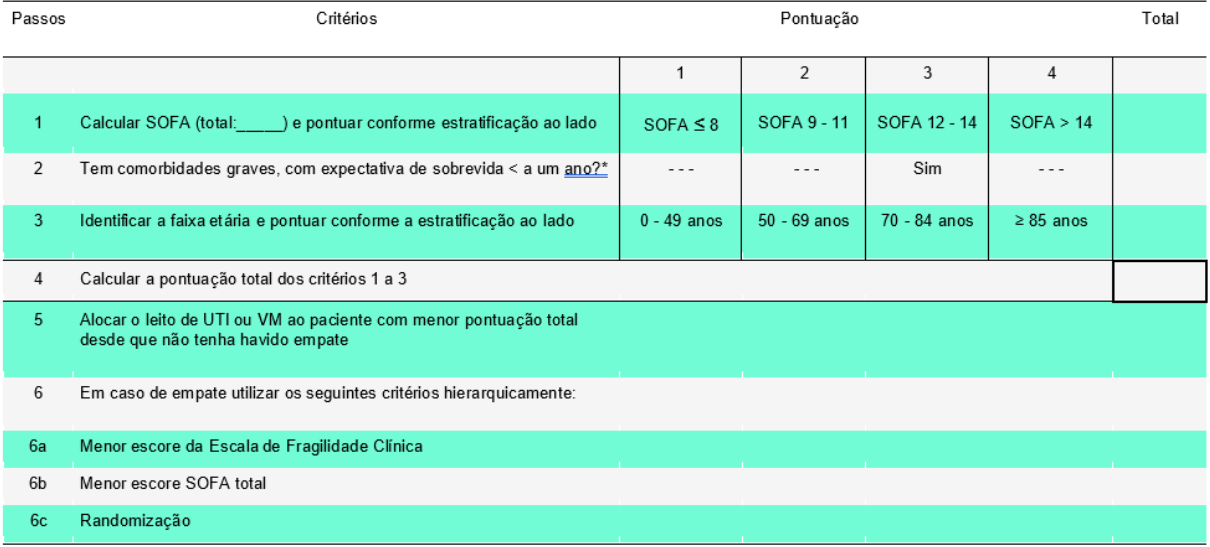
\includegraphics[scale=0.5]{img/Tabela de pontuacoes e criterios.png}
    \centering
    \caption{Passos do modelo de triagem AMIB/ABRAMEDE \cite{kretzer2020recomendaccoes}}
    \label{Passos-modelo-triagem-AMIB-ABRAMEDE}
\end{figure}

Para um entendimento melhor do porque foi escolhido esses critérios pela equipe do AMIB, será descrito o que são os critérios.

\subsubsection{CRITÉRIO 1 - SEQUENTIAL ORGAN FAILURE ASSESSMENT (SOFA)}

O SOFA é o primeiro critério do protocolo AMIB, ele avalia objetivamente o avanço de uma disfunção orgânica em pacientes que apresentam alguma infecção, bem como a mortalidade diante de um estado de saúde crítico de um indivíduo, avaliando seis sistemas diferentes a partir de diversos exames clínicos e laboratoriais, e prediz a mortalidade de pacientes com sepse (presença de disfunção orgânica que ameaça a vida, por conta de uma resposta exacerbada a uma infecção) a partir da pontuação \cite{lambden2019sofa}.

Cada um dos seis sistemas, representam um sistema do órgão, sendo atribuído um valor entre zero e quatro pontos, sendo zero o valor representando que o sistema está normal, e quatro representando que o sistema está em um alto grau de disfunção ou falência. A soma dos pontos do escore SOFA varia entre zero e vinte e quatro (0-24), existindo uma relação entre a pontuação do SOFA com uma porcentagem referente à mortalidade do paciente, a tabela a seguir demonstra essa relação:

\begin{center}
    \begin{tabular}{l r r r}
        \hline
        PONTUAÇÃO SOFA & MORTALIDADE EM X\% \\
        \hline
            0–6	& $\leq 10$\% \\
            7–9	& 15–20\% \\
            10–12 & 40–50\% \\
            13–14 & 50–60\% \\
            15 & $\geq80$\% \\
            15–24 & $\geq90$\% \\
        \hline
    \end{tabular}
\end{center}


Os seis sistemas são avaliados e recebem uma pontuação, são eles: O sistema respiratório, cardiovascular, hepático, renal, neurológico e de coagulação. A pontuação deve ser calculada 24 horas após a admissão e a cada 48 horas depois o que  justifica o termo “sequencial” do nome da pontuação.

\begin{enumerate}
    \item Sistema respiratório: avaliado a partir de dados obtidos através de gasometria arterial, coletado através de um exame de sangue em uma artéria, sendo avaliado da razão entre PaO2/FiO2, os gases presentes no sangue, como o oxigênio o gás carbônico \cite{mota2010disturbios}. Abaixo de 400, 1 ponto no SOFA. Abaixo de 300, 2 pontos. A pontuação é 3 quando o paciente está em suporte ventilatório com a PaO2/FiO2 abaixo de 200, e ele recebe a pontuação máxima quando a relação tem resultado menor que 100mmHg com suporte ventilatório.
    
    \item Sistema coagulação: avaliado a partir do exame de contagem de plaquetas/trombócitos no sangue (plaquetograma). O valor considerado de referência, ou seja, que não pontua no score SOFA, é 150.000/mm³. Os valores de corte para as pontuações de 1 a 4, respectivamente, são abaixo de 150, 100, 50 e 20.
    
    \item Sistema hepático: realizada com o exame de bilirrubinas totais para avaliar o funcionamento do fígado, é uma substância alaranjada produzida quando o fígado decompõe glóbulos vermelhos velhos \cite{lambden2019sofa}.
    
    \item Sistema cardiovascular: o paciente que apresenta hipotensão e necessidade de droga vasoativa (DVA) é quem pontua nesta parte do score. É mensurado a partir da pressão arterial média, que recebe 1 ponto em caso de PAM<70mmHg. A partir do 2º ponto, é considerado o uso de DVA – 2 pontos se uso de dopamina<5 ou dobutamina em qualquer dose;  3 pontos em caso de uso de dopamina, noradrenalina ou adrenalina em doses mais baixas, e em caso de aumento da dosagem das DVAs, o paciente recebe a pontuação de 4 pontos \cite{nakashima2020intervindo}.
    
    \item Sistema neurológico: recebe avaliação a partir da escala de coma de Glasgow.
    
    \item Sistema renal: para a avaliação é considerado dois parâmetros: 1-creatinina; 2-débito urinário. A creatinina se demonstra alterada a partir de 1,2mg/dL, pontuando 1 até 1,9mg/dL. Valores de 2,0 a 3,4mg/dL pontuam 2, enquanto o paciente que apresenta diurese menor que 500 ml por dia OU creatinina de 3,5 a 4,9mg/dL pontua 3. Quando a diurese é inferior a 200 ml por dia ou a creatinina é superior a 5, o paciente recebe o score máximo \cite{lambden2019sofa}.
    
\end{enumerate}

\subsubsection{CRITÉRIO 2 - SUPPORTIVE AND PALLIATIVE CARE INDICATORS TOOL (SPICT)}

A ferramenta SPICT-BR é o segundo critério do protocolo AMIB, é uma lista de indicadores gerais de deterioração clínica e de indicadores de gravidades de doenças específicas: doenças
cardiovasculares, doenças renais, respiratórias, hepáticas, câncer, doenças neurológicas e
demências e fragilidades \cite{rodriguez2021pergunta}. Para que haja a indicação de cuidado paliativo do paciente necessita pontuar pelo menos 02 ou mais dos indicadores gerais e 01 indicador específico. O SPICT-BR foi traduzido e validado para utilização em pacientes brasileiros em abril de 2016. A Pergunta Surpresa, corresponde ao questionamento – “Você acredita que o seu paciente tem expectativa de vida menor do que 12 meses?”, direcionado à equipe de saúde, mas especificamente, ao médico assistente. Se a resposta for “Sim”, o paciente se beneficiará dos Cuidados Paliativos.

Para o protocolo AMIB, se caso o paciente estiver com a pergunta surpresa como "Sim" receberá 3 pontos no total, caso contrário não soma.

\subsubsection{CRITÉRIO 3 - EASTERN COOPERATIVE ONCOLOGY GROUP (ECOG)}
O Eastern Cooperative Oncology Group (ECOG) é o terceiro critério do protocolo AMIB, é um
instrumento validado e amplamente utilizado em oncologia e que busca quantificar a capacidade funcional física e capacidade de independência e auto-cuidado do paciente. A inferência é que quanto pior o PS do paciente menor sua reserva fisiológica e piores os desfechos clínicos.

A coleta desta medida deve ser referente à performance que o paciente exiba nas duas a quatro semanas que antecederam a internação de maneira a excluir o fator confundidor da presença de doença aguda que possa ter se iniciado nas duas semanas imediatamente anteriores a internação hospitalar. Não recomendamos o uso deste critério, sem uma avaliação clínica individualizada, a pacientes portadores de deficiências físicas de longa data e que apresentem uma boa condição de adaptação \cite{pinto2000physician}.

\section{ALGORITMO PARA GERAÇÃO DE DADOS}

O roteiro do código se baseará totalmente no protocolo da Associação de Medicina Intensiva Brasileira (AMIB), de alocação de recursos em esgotamento durante a pandemia por COVID-19 \cite{kretzer2020recomendaccoes}, considerando que existem oito variáveis clínicas a serem avaliados para aplicar os três critérios do protocolo, serão denotados de $a_1$ até $a_8$:

\[
    \begin{split}
        a_1 &\in \{0, 1, 2, 3, 4\}\text{, sendo o critério neurológico} \\
        a_2 &\in \{0, 1, 2, 3, 4\}\text{, sendo o critério respiratório} \\
        a_3 &\in \{0, 1, 2, 3, 4\}\text{, sendo o critério cardiovascular} \\
        a_4 &\in \{0, 1, 2, 3, 4\}\text{, sendo o critério coagulatório} \\
        a_5 &\in \{0, 1, 2, 3, 4\}\text{, sendo o critério hepático} \\
        a_6 &\in \{0, 1, 2, 3, 4\}\text{, sendo o critério renal} \\
        a_7 &\in \{0, 3\}\text{, sendo o critério de comorbidades (SPICT) } \\
        a_8 &\in \{0, 1, 2, 3, 4\}\text{, sendo o critério da escala de status de desempenho (ECOG)} \\
    \end{split}
\] 

O primeiro critério que compõe a pontuação total do protocolo, é o SOFA, demonstrado nas variáveis de $a_1$ até $a_6$, que conforme os valores aferidos do paciente são atrelados a pontos para cada variável do SOFA, resultando em um somatório SOFA final, quantificando entre zero e quatro pontos.

Em seguida o modelo do protocolo AMIB levanta o critério de comorbidades graves do paciente, o qual deve ser analisado a situação de cuidados paliativos juntamente com variáveis definidas na ferramenta SPICT, se caso a Pergunta Surpresa: “Você acredita que o seu paciente tem expectativa de vida menor do que 12 meses?” for respondida como “Sim” será pontuado como três pontos no total do calculo AMIB.

Para compor o último critério do protocolo AMIB, calcula-se a escala de status de desempenho utilizando o ECOG, que busca quantificar a capacidade funcional física e capacidade de independência e auto-cuidado do paciente, quantificando entre zero e quatro pontos.

Portanto para calcular a pontuação total dos três critérios levanta-se a seguinte expressão matemática:

\[
\begin{split}
    s &= \sum_{n=1}^{6} a_n\text{, sendo o SOFA} \\
    C_1 &= \begin{cases}
        1, \text{se } & s \le 8 \\
        2, \text{se } 8 < & s \le 11 \\
        3, \text{se } 11 < & s \le  14 \\
        4, \text{se } 14 < & s \\
    \end{cases} \\
    C_2 &= \begin{cases}
        0, \text{se } & a_7 \neq "Sim" \\
        3, \text{se } & a_7 \equiv "Sim" \\
    \end{cases} \\
    C_3 &= \begin{cases}
        1, \text{se } a_8 = 1 \\
        2, \text{se } a_8 = 2 \\
        3, \text{se } a_8 = 3 \\
        4, \text{se } a_8 = 4 \\
    \end{cases} \\
    t &= C_1 + C_2 + C_3 \\
\end{split}
\] 

Portanto, dados dois pacientes, $p_1$ e $p_2$, o protocolo decide entre os dois primeiramente comparando o valor de $t$ calculado para cada um, se  $t_{p_1}$ for menor que $t_{p_2}$ o protocolo prescreve que a preferência na obtenção do leito seja de $p_1.$ sendo a recíproca naturalmente verdadeira.

Se $t$ for igual para $p_1$ e $p_2$, o protocolo sugere é realizada a comparação de ambos usando $s$. Se caso $t$ e $s$ serem iguais para $p_1$ e $p_2$, utiliza-se o julgamento clínico será da equipe de triagem, ou seja, um ou mais profissionais decidirão entre ambos, para qual utilizará um leito de UTI.


\section{RESULTADOS EXPERIMENTAIS}

Após mapear as variáveis com os critérios do protocolo AMIB, é possível realizar uma classe denominada "Paciente" que contém oito variáveis já descritas no modelo matemático, de forma a gerar dados sintéticos para validação do modelo sugerido.

A criação de um algoritmo desenvolvido para este artigo com as $a_1$ até $a_8$ e os critérios $C_1$, $C_2$ e $C_3$ resulta em saídas onde é escolhido um paciente sem ocorrer empate, ou é realizado um empate da soma total, porém o critério de desempate SOFA resolve, porém para esse artigo, decidiu-se forçar casos clínicos em que o protocolo seja incapaz de fornecer distinção relevante a respeito de priorização de paciente relação a outro, no caso em que o protocolo sugere julgamento clínico, voltando a total responsabilidade para pessoas.
Notadamente, é possível desenhar uma função $\alpha \in [0, 1]$ que informe o grau de certeza com o qual o protocolo determina a prioridade:
% REVISAR ESSE CÁLCULO----
\[
\alpha = \begin{cases}
    \frac{t_{p_1} - t_{p_2}}{\max_t - \min_t}, \text{se } t_{p_1} - t_{p_2} \neq 0 \\
    \frac{a_{7p_1} - a_{7p_2}}{\max_{a_7} - \min_{a_7}}, \text{se } a_{7p_1} - a_{7p_2} \neq 0 \\
    \frac{a_{8p_1} - a_{8p_2}}{\max_{a_8} - \min_{a_8}}, \text{se } a_{8p_1} - a_{8p_2} \neq 0 \\
    \frac{s_{p_1} - s_{p_2}}{\max_s - \min_s}, \text{se } s_{p_1} - s_{p_2} \neq 0 \\
    0, \text{se o protocolo julgamento clínico da equipe de triagem}
\end{cases}
\] 
% REVISAR ESSE CÁLCULO----

Com o objetivo deste artigo sendo minimizar $\alpha$, será trivial considerando o caso de dois pacientes com todos os critérios idênticos, mas esse caso foge do que é desejável, pois não são cabíveis quaisquer outros argumentos quanto a priorização.
Para tando, utiliza-se a noção de inércia ($i$) como medida de homogeneidade, de forma que valores menores de $i$ implicam em conjuntos de pacientes mais homogêneos.
A inércia pode ser calculada como o quadrado da distância de cada membro do conjunto para o centro de gravidade do conjunto.

\[
I = \sum_{p \in P}d(p, c)^2
\] 

Considerando $P$ o conjunto de pacientes, $c$ o centro de massa desse conjunto e $d$ a distância euclideana, é possível a construção de um conjunto de dados que maximize a obtenção de quais são os critérios de decisão de um julgamento clínico, presumindo que utilize o protocolo AMIB. Para tanto, qualquer que seja o conjunto de pacientes que o médico ordenará, esse deve maximizar a inercia e minimizar alfa.

Considerando uma função de qualidade $\frac{I}{\alpha}$, realiza-se uma busca por um conjunto especificado de dez pacientes da seguintes forma:

É construído um novo paciente $P$ escolhendo um ponto nesse espaço de nove dimensões, nesse processo são feitas validações de $a_1$ até $a_9$ de forma que pertence aos conjuntos definidos, validando as seguintes regras clínicas:

\[
\begin{split}
    \begin{cases}
    R_1: a_1 \and a_6 &\in \{0, 1, 2, 3, 4\} \\
    R_2: a_7 &\in \{0, 3\} \\
    R_3: a_8 &\in \{0, 1, 2, 3, 4\} \\
    %Quando Respiratório com ventilação mecânica (3 ou 4) o Glasgow tem que ser 3 ou 4
    R_4: a_1 \ge 3 \implies a_3 \ge 3 \\
    \end{cases}
\end{split}
\]

No mesmo algoritmo é construído um conjunto de 10 pacientes, para o conjunto é calculada a função $\frac{I}{\alpha}$ assim como os 10 subconjuntos de 9 elementos.
No subconjunto com maior $\frac{I}{\alpha}$ será complementado com um novo paciente gerado e validado se o $\frac{I}{\alpha}$ ainda é maior $\frac{I}{\alpha}$ do conjunto original.

O registro hipotético validado na função com maior valor é utilizado para a persistência da informação, o processo fica em um laço de repetição por dez mil vezes, pré programado no código.

Dessa forma o algoritmo fornece um conjunto de paciente homogêneos e em que o protocolo AMIB sugere que seja utilizado um julgamento clínico pelos profissionais.


Com uma geração de mil registros de pacientes hipotéticos, percebe-se que há uma homogeneidade entre a soma do SOFA, ou seja, a porcentagem da mortalidade com os pacientes gerados. Na imagem abaixo podemos perceber que existe similaridades entre os conjuntos de Pacientes, mesmo quando possuem valores diferentes.

\begin{figure}[!htb]
    \centering
    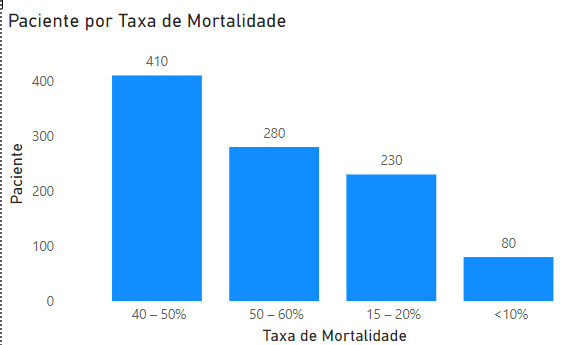
\includegraphics[scale=0.9]{img/Taxa de Mortalidade2.png}
    \centering
    \caption{Paciente sintético por taxa de mortalidade.}
    \label{Paciente-gerado-taxa-mortalidade}
\end{figure}

Entende-se que desses mil pacientes gerados sinteticamente, maior parte tem uma taxa de mortalidade de 40 a 50\%, o que analisando os dados de algumas amostras, tem sentido com a realidade de pessoas que necessitam de leito de UTI.

Para uma visualização mais detalhada dos mesmos dados, mostra-se o resultado da soma do SOFA em relação aos pacientes. Não foi demonstrado o somatório total dos pontos porque o algoritmo forçou a soma do total e do SOFA de forma idêntica, fazendo com que resulte o mesmo gráfico.

\begin{figure}[!htb]
    \centering
    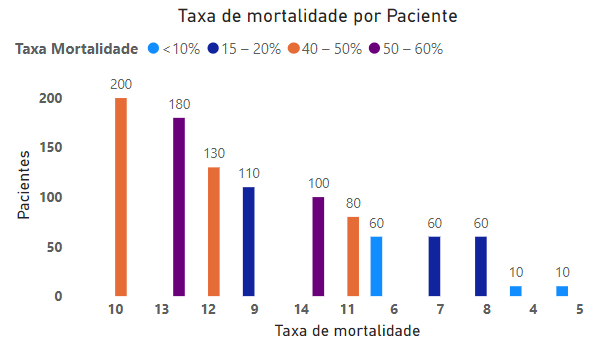
\includegraphics[scale=0.9]{img/Taxa de Mortalidade.png}
    \centering
    \caption{Paciente sintético por soma do SOFA, legenda taxa de mortalidade.}
    \label{Paciente-gerado-por-SOFA-legenda-taxa-mortalidade}
\end{figure}


Quando colocado cada paciente comparando com todos, temos um milhão de registros simulando decisões em pares com cada paciente, de forma simplificada o algoritmo foi desenvolvido para gerar cem conjuntos de 10 pacientes, esses contém o mesmo total de pontos AMIB e o mesmo SOFA, ou seja, esses 10 pacientes devem ser julgado por um médico. 

Diante dessa massa de dados, de mil registros, o algoritmo comparou cada registro com os outros novecentos e noventa e nove, para definir qual é o paciente prioritário a cada par, dessa comparação, gerou uma massa de dados de um milhão de registros a qual o protocolo AMIB classificou em 1, se for o primeiro paciente da dupla o mais prioritário, em 2 se for o segundo paciente e em 0 (zero) se não consegue definir um mais prioritário conforme as regras já citadas.
Na imagem abaixo notamos que somente 10\% das comparações as regras do protocolo AMIB não consegue decidir.

\begin{figure}[!htb]
    \centering
    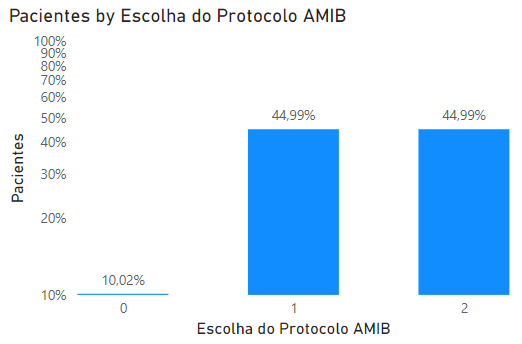
\includegraphics[scale=0.9]{img/comparação.png}
    \centering
    \caption{Decisão do protocolo AMIB comparando a massa de dados. }
    \label{Decisão-de-pacientes-1-2-0}
\end{figure}



\clearpage

\section{CONSIDERAÇÕES FINAIS}

Em um cenário de crise na saúde pública, nota-se a importância de utilizar um modelo de triagem para decisão clínica. Um protocolo criado pela Associação de Medicina Intensiva Brasileira, que tem dentre os objetivos, proteger os profissionais do peso moral e jurídico da decisão, com transparência do processo de decisão comprova-se que diante de dados clínicos gerados sinteticamente, e o algoritmo desenvolvido que o protocolo AMIB consegue discernir entre dois paciente em 90\% dos casos

\section{PRÓXIMAS ETAPAS}

Interessante usar colapso de função de onda \ldots

Algoritmo genético para geração \ldots


\section{REFERÊNCIAS BIBLIOGRÁFICAS}

\bibliographystyle{sbc}
\bibliography{sbc-template}

\end{document}

